\documentclass{article}
\usepackage{url,amsfonts, amsmath, amssymb, amsthm, graphicx, braket, fancyhdr, physics, mathtools}
\graphicspath{ {./QM_Images/} }
% Page layout
\setlength{\textheight}{8.75in}
\setlength{\columnsep}{2.0pc}
\setlength{\textwidth}{6.5in}
\setlength{\topmargin}{0in}
\setlength{\headheight}{0.0in}
\setlength{\headsep}{0.0in}
\setlength{\oddsidemargin}{0in}
\setlength{\evensidemargin}{0in}
\setlength{\parindent}{1pc}

% Commands
\newcommand{\RNum}[1]{\uppercase\expandafter{\romannumeral #1\relax}}

\usepackage[a4paper,margin=2cm,portrait, headsep=24pt, headheight=2cm]{geometry}
\usepackage{enumitem}

% Header
\pagestyle{fancy}
\fancyhf{}
\rhead{Page \thepage}
\chead{Quantum Mechanics DE}
\lhead{James Natoli}
\rfoot{}

\begin{document}
% suppress header on first page
\thispagestyle{empty}
%%% Title Stuff
\begin{center}\Large \textbf{Quantum Mechanics Departmental Exam} \\
\normalsize James Natoli \\  January 2021
\end{center}

%%%%%%%%%%%%%%%%% Problem 1 %%%%%%%%%%%%%%%%%
\section*{Problem 1} 
A particle is in the \underline{ground} state of an infinite square well. That is \\
\[ V(x) = \begin{cases} 
      0 & 0\leq x\leq L \\
      \infty & \text{otherwise}
   \end{cases}
\]
At t=0 the wall is \underline{suddenly} moved to x=2L -- this happens \underline{very fast}, approximately instantaneously.
\begin{enumerate}[label=\alph*)]
	%%% Part (A)
	\item Calculate the probability that long after t=0 the system is in the ground state of the new potential.
	%%% Part (B)
	\item How fast must the change take place for this "instantaneous" assumption to be good?
\end{enumerate}
%%% Solution
\section*{\textit{Solution}} 
\begin{enumerate}[label=\alph*)]
	% PART (A)
	\item We know our standard initial ground state of Infinite Square Well (ISW) and the energy are given by (derivation in Griffiths 2.2)
	\[\psi^L_n(x) = \sqrt\frac{2}{L}\sin\left(\frac{n\pi x}{L}\right), E^L_n = \frac{n^2\pi^2\hbar^2}{2mL^2}\]
	And for after the shift, when ($L \rightarrow 2L$)
	\[ \psi^{2L}_n(x) = \sqrt\frac{1}{L}\sin\left(\frac{n\pi x}{L}\right), E^{2L}_n = \frac{n^2\pi^2\hbar^2}{8mL^2}\]
	Let's now project our initial state in to our new (2L) basis, or recalling that we can express any function as a linear combination of ISW basis states
	\[\psi^L_1(x) = \sum_n^{\infty} c_n \psi^{2L}_n(x) \]
	Now use the Fourier Trick, multiplying both sides by $\bra{\psi^{2L}_n(x)}$ and integrating. 
	\begin{align}		
	\bra{\psi^{2L}_1(x)}\ket{\psi^L_1(x)} = \sum_n^{\infty} c_n \delta_{2L, L} &= c_1 \\
	\int \sqrt\frac{1}{L}\sin\left(\frac{\pi x}{2L}\right)\sqrt\frac{2}{L}\sin\left(\frac{\pi x}{L}\right) \,dx &= c_1 \\
	\sqrt\frac{2}{L} \int_0^L 2\sin^2\left(\frac{\pi x}{2L}\right)\cos\left(\frac{\pi x}{2L}\right)\,dx &= c_1 \\
	\text{where here we used } \sin(2x) = 2\sin(x)\cos(x) \\
	\frac{2\sqrt{2}}{L} \int_0^L \left(\frac{2L}{\pi}\right) u^2 \,du &= c_1 \\
	\text{where here we used } u = \sin\left(\frac{\pi x}{2L}\right), du = \left(\frac{2L}{\pi}\right)\cos\left(\frac{\pi x}{L}\right) \\ 
	\frac{4\sqrt{2}}{\pi}\left( \frac{\sin^3\left(\frac{\pi}{2}\right)}{3} \right) &= c_1 \\
	\frac{4\sqrt{2}}{3\pi} &= c_1
	\end{align}
	We now recall that the probability of a transition is $|c_n|^2$, so
	\[ \boxed{P_1 = |c_1|^2 = \frac{32}{9\pi^2} \approx 0.36 } \]
	% PART (B)
	\item To find the time minimum time interval for this 
	instantaneous assumption to be valid, we recall the lesser known twin in the Heisenberg Uncertainty Principle
	\[ \Delta E \Delta t \geq \frac{\hbar}{2} \]
	\begin{align}
	\text{where } \Delta E &= E^{2L}_1 - E^L_1 \\ 
	&= \frac{\pi^2\hbar^2}{2mL^2} - \frac{\pi^2\hbar^2}{8mL^2} \\
	&= \frac{3\pi^2\hbar^2}{8mL^2}
	\end{align}
	\[ \text{and so }\frac{3\pi^2\hbar^2}{8mL^2}\Delta t \geq \frac{\hbar}{2} \]
	\[ \boxed{ \Delta t \geq \frac{4mL^2}{3\pi^2\hbar} } \]
\end{enumerate}

%%%%%%%%%%%%%%%%% Problem 2 %%%%%%%%%%%%%%%%%
\section*{Problem 2} 
% Problem Statement
\begin{enumerate}[label=\alph*)]
	\item % PART (A)
	Consider a particle of mass, $\textit{m}$, and energy E, in a one-dimensional potential as shown. Derive expressions from which the eigenvalue E can be determined for the even-parity and the odd-parity solutions.
	\item % PART (B)
	Describe briefly how one would obtain the numerical value of E for the even-parity solutions.
	\begin{figure}[h]
	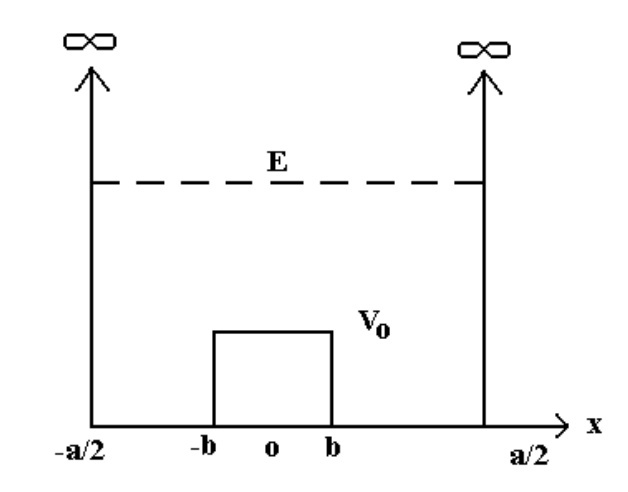
\includegraphics[scale=0.25]{P2}
	\centering
	\end{figure}
\end{enumerate}
%%% Solution Here
\section*{\textit{Solution}} 
\begin{enumerate}[label=\alph*)]
	% PART (A)
	\item This is basically the ISW but with a brick at the bottom. To begin, we split the well in to 3 regions: I from $\frac{-a}{2}$ to -b, II from -b to b, and III from b to $\frac{a}{2}$. We then use our standard ISW solutions, which are a linear combination of trig functions	.	\begin{align}
		\psi_{\RNum{1}}(x) &= A\cos(k_{1}x) + B\sin(k_{1}x) \\ 
		\psi_{\RNum{2}}(x) &= C\cos(k_{2}x) + D\sin(k_{2}x) \\ 
		\psi_{\RNum{3}}(x) &= A\cos(k_{1}x) + B\sin(k_{1}x) 
	\end{align}
	where our k's are
	\[ k_1 = \frac{\sqrt{2mE}}{\hbar} \text{ and } k_2 = \frac{\sqrt{2m(E-V_0)}}{\hbar} \]
	Lets look first at $\textbf{even } (f(x) = f(-x))$ solutions, so B = D = 0 and only caring abut the cosines. We now enforce our boundary conditions at $\pm b$. But we can get away with only looking at $+b$ first. Remember that the standard boundary conditions are $\textbf{(A)}$ function is continuous and, $\textbf{(B)}$ derivative is continuous.
	
	\text{Applying } \textbf{(A)}
	\begin{align}
	\psi_{\RNum{2}}(x) &= \psi_{\RNum{3}}(x) \\ 
	C\cos(k_{2}b) &= A\cos(k_{1}b) 
	\end{align}
	\text{and applying } \textbf{(B)} \\
	\begin{align}
	\frac{ \partial }{\partial x} \psi^e_{\RNum{2}} \Bigr\rvert_{x = b} &= \frac{ \partial }{\partial x} \psi^e_{\RNum{3}} \Bigr\rvert_{x = b} \\ 
	k_2C\sin(k_2b) &= k_1A\sin(k_2b)
	\end{align}
	Lastly, we divide (18) by (16) to get 
	\[ \boxed{ k_2\tan(k_2b) = k_1\tan(k_1b) } \]
	
Now we'll do the same process for the odd solutions, so A = C = 0, only caring about the sines. Applying the boundary conditions at b, we get 
	\[ \boxed{ k_2\cot(k_2b) = k_1\cot(k_1b) } \]
	% PART (B)
	\item To obtain E for just the even parity solutions, you would graph $k_2\tan(k_2b)$ and  $k_1\tan(k_1b)$, and the point of intersection would allow you to solve for E
\end{enumerate}

%%%%%%%%%%%%%%%%% Problem  3 %%%%%%%%%%%%%%%%%
\section*{Problem } 
% Problem Statement
\begin{enumerate}[label=\alph*)]
	% PART (A)
	\item Consider a helium-like ion. The two electrons are in the 2p and 3p states. The energy levels will have definite total angular momentum $(\vec{J} = \vec{L} + \vec{S})$. \underline{What J-values} can occur and \underline{how many energy levels of each J} can there be?
	% PART (B)
	\item How do your answers change if the electrons are both in 3p states?
\end{enumerate}
%%% Solution Here
\section*{\textit{Solution}} 
\begin{enumerate}[label=\alph*)]
	% PART (A)
	\item Our friendly atom has both of it's electrons in the p states, so $l_1 = l_2 = 1$ and $s_1 = s_2 = \pm \frac{1}{2}$. Let's recall our definitions of $\vec{L}$ and $\vec{S}$
	\begin{align}
	\vec{L} &= |l_1- l_2|, \cdots integers \cdots |l_1 + l_2| \\ 
	\vec{L} &= 0, 1, 2 \\ 
	\vec{S} &= |s_1- s_2|, \cdots integers \cdots |s_1 + s_2| \\ 
	\vec{S} &= 0, 1
	\end{align}
This means we can have $\boxed{\vec{J} = 0, 1, 2, 3}$. Quick aside on the spins, we don't actually know what the spin of the individual electrons are until we measure them, but it doesn't matter. any combination of $\pm\frac{1}{2}$ gives us the same values for $\vec{S}$, the total spin. The second part of the question, asking about how many energy levels of each $\vec{J}$ there can be is asking about the \underline{degeneracy}, which you're kind of just supposed to know is $2\vec{J} +1$. I'm sure there's a derivation somewhere, but like is it really that important? Probably not.

\item Now they want to know what would happen if both electrons are hanging out in the 3p state. The spin is important now because although they are indistinguishable, we know they are opposite due to the Pauli Exclusion principle, so $\vec{S} = 0$ and $\boxed{\vec{J} = 0, 1, 2}$, but the degeneracies are the same.
	
\end{enumerate}

%%%%%%%%%%%%%%%%% Problem  4 %%%%%%%%%%%%%%%%%
\section*{Problem 4}	 
% Problem Statement
In precise treatments of hydrogen-like atoms, the finite size of the nucleus has to be included in the calculation of the electronic energy levels. Assume the nucleus to be a sphere with a uniform charge distribution.
\begin{enumerate}[label=\alph*)]
	\item % PART (A)
	Write down the correction to the potential experienced by the electron.
	\item % PART (B)
	Calculate the first order correction to the energy.
\end{enumerate}
%% Solution Here
\section*{\textit{Solution}} 
\begin{enumerate}[label=\alph*)]
	\item % PART (A)
	From E\&M, you're kind of just supposed to know that potential of a sphere is 
	\[ V_{sphere} (r) = \frac{kQ}{r} = \frac{1}{4\pi\epsilon_0} \cdot \frac{Q}{r}\]
	Probably best to memorize this, but I'm sure Griffiths/Jackson have a derivation.
	\item  % PART (B)
	Wading in to this puppy now, we're gonna be using first order perturbation theory. I'm just gonna use the formula's which are good to know but look in Griffiths' chapter 6 if you want the derivation.
	\[
	E^1_n = \bra{\psi^0_n}H'\ket{\psi^0_n}
	\]
I'm gonna assume the ground state, not sure if that's right but it sure does make it simpler
	\begin{align}
	&= \int_\infty \psi^{*}_{100}(r,\theta,\phi)\left(\frac{kQ}{r}\right)\psi_{100}(r,\theta,\phi)r^2\sin(\theta)\,drd\theta d\phi \\ 
	\text{using } &\psi^{*}_{100}(r,\theta,\phi) = \frac{1}{\sqrt{\pi a^3}}e^{-r/a} \text{ which is good to memorize} \\
	&= \frac{kQ}{\pi a^3} \int_0^{2\pi}\,d\phi\int_0^{\pi} \sin(\theta)\,d\theta\int_0^\infty e^{-r/a}re^{-r/a} \,dr \\ 
	&= \frac{4kQ}{a^3} \int_0^\infty re^{-2r/a} \,dr \\ 
	\text{using }& \int_0^\infty xe^{cx} \,dx = \frac{xe^cx}{c} - \frac{e^cx}{c^2} \\
	&= \frac{4kQ}{a^3} \left( \frac{re^{\frac{-2r}{a}}}{-2/a} - \frac{e^{\frac{-2r}{a}}}{4/a^2}\right]_0^R \\ 
	&= \frac{4kQ}{a^3} \left( \frac{-aRe^{\frac{-2R}{a}}}{2} - \frac{a^2e^{\frac{-2R}{a}}}{4}\right) - \frac{a^2}{4}
	\end{align}
	I think this is the answer? Take Q = e for the electron charge. I changed the bounds on the r integral from 0 $\rightarrow \infty$ to 0 $\rightarrow R$ because the wave function is zero outside of that radius, but that assumption could be incorrect.
\end{enumerate}

%%%%%%%%%%%%%%%%% Problem  5 %%%%%%%%%%%%%%%%%
\section*{Problem 5} 
% Problem Statement
Two indistinguishable spin-$\frac{1}{2}$ particles of mass $\textit{m}$ move in a 1D simple harmonic oscillator (HO) with frequency $\omega_0$. Using center-of-mass and relative coordinates, answer the following:
\begin{enumerate}[label=\alph*)]
	\item % PART (A)
	What is the spectrum of singlet states? of triplet states? What is the ground state of the system?
	\item % PART (B)
	Now let's assume that the particles have charge $\textit{q}$ --- but do not interact with each other --- and are exposed to the time-dependent perturbation
	\[
	H' = -q\mathbf{E_0}x_1e^{-\left(\frac{t}{\tau}\right)^2}\cos\omega t - q\mathbf{E_0}x_2e^{-\left(\frac{t}{\tau}\right)^2}\cos\omega t
	\]
	Take $\textit{q}$, $\mathbf{E_0}$ and $\tau$ to be real, positive constants. If the system is initially in the ground state from (a), $\ket{i} = \ket{n_{1}^{(i)},n_{2}^{(i)}}$, calculate the probability (in first order perturbation theory)
	\[
	P_{if}(t) = \frac{1}{\hbar^2} | \int_{-\infty}^{\infty}dt\bra{f}H'(t)\ket{i}e^{\frac{i(\epsilon_{f} - \epsilon_{t})t}{\hbar}}|^2
	\]
	for finding the system in a state $\ket{f}=\ket{n_{1}^{(f)},n_{2}^{(f)}}$ at time t. \\
	Potentially useful information:
	\[ \text{i)}
		\int_{-\infty}^{\infty}dx\:x^{2n}e^{-x^2} = (-1)^n \frac{d^n}{d\beta^n}\int_{-\infty}^{\infty}dx\:e^{-\beta x^2} |_{\beta = 1} = (-1)^n \frac{d^n}{d\beta^n} \sqrt{\frac{\pi}{\beta}} |_{\beta=1}
	\]
	\[ \text{ii)}
		\bra{k}x\ket{n} = \sqrt{\frac{\hbar}{m\omega}}\left[ \sqrt{\frac{n}{2}} \delta_{k,n-1}+\sqrt{\frac{n+1}{2}}\delta_{k,n+1}\right]
	\] 
	\hspace{3.5 cm} $\bra{k}x\ket{0} = \sqrt{\frac{\hbar}{2m\omega}}\delta_{n,1}$
\end{enumerate}
%% Solution Here
\section*{\textit{Solution}} 
\begin{enumerate}[label=\alph*)]
	\item % PART (A)
	First, we need to know that a \underline{spectrum} is the \underline{allowed energy values}. We also need to recall some important info about singlet and triplet states
	\[ \text{singlet } = \text{ anti-symmetric spin state} \]
	\[ \text{triplet } = \text{ symmetric spin state} \]
	This can be derived from their definitions, but that is good to memorize. Further reading in Griffiths pg. 185-186. Spin-$\frac{1}{2}$ particles are by definition overall anti-symmetric, so a singlet must have a symmetric space function and a triplet must have an anti-symmetric space function. Lets look first at \underline{singlet}
	\begin{align}
		\psi(x_1,x_2) &= \frac{1}{\sqrt{2}}\left[ \psi_{n1}(x_1) \psi_{n2}(x_2) + \psi_{n1}(x_2) \psi_{n2}(x_1)\right],  n_1 \neq n_2  \\
		\psi(x_1,x_2) &= \psi_{n1}(x_1) \psi_{n2}(x_2), n_1 = n_2 \\
		E &= \hbar\omega, 2\hbar\omega, 3\hbar\omega, \dots
	\end{align}
	(30) and (31) both satisfy $ \psi(x_1,x_2) = \psi(x_2,x_1)$, which is the condition for symmetry \\
	Now consider the \underline{triplet}, which requires an anti-symmetric space function, so our only option is $\dots$
	\begin{align}
		\psi(x_1,x_2) &= \frac{1}{\sqrt{2}}\left[ \psi_{n1}(x_1) \psi_{n2}(x_2) - \psi_{n1}(x_2) \psi_{n2}(x_1)\right],  n_1 \neq n_2 \\ 
		E &=  2\hbar\omega, 3\hbar\omega, \dots
	\end{align}
	The energy values came from recalling that for HO $\dots$
	\[ E_n = (n+\frac{1}{2})\hbar\omega \Rightarrow E_{n1,n2} = (n_2+n_2+\frac{1}{2}+\frac{1}{2})\hbar\omega = (n_2+n_2+1)\hbar\omega \]
	The last part of (a) asks us for the ground state, which is just the state that corresponds to the lowest energy so
	\begin{align}
		\text{Singlet} \rightarrow \psi(x_1,x_2) &= \psi_{0}(x_1) \psi_{0}(x_2)\cdot\chi_{sing} \\
		\text{Triplet} \rightarrow \psi(x_1,x_2) &= \frac{1}{\sqrt{2}}\left[ \pm \psi_{0}(x_1) \psi_{1}(x_2) \mp \psi_{1}(x_1) \psi_{0}(x_2)\right]\cdot\chi_{trip}
	\end{align}
	where $\chi_{sing}$ and $\chi_{trip}$ denote the spin states (spinors?)
	\item Now we're asked to consider what happens if the particles are charged but non interacting
	This is when we use our handy dandy first order perturbation theory, so we're told system is originally in the ground state (lowest energy state) and remember that
	\[
	H' = -q\mathbf{E_0}x_1e^{-\left(\frac{t}{\tau}\right)^2}\cos\omega t - q\mathbf{E_0}x_2e^{-\left(\frac{t}{\tau}\right)^2}\cos\omega t = -q\mathbf{E_0}e^{-\left(\frac{t}{\tau}\right)^2}\cos\omega t (x_1 + x_2)
	\]
	and 
	\[
	P_{if}(t) = \frac{1}{\hbar^2} | \int_{-\infty}^{\infty}dt\bra{f}H'(t)\ket{i}e^{\frac{i(\epsilon_{f} - \epsilon_{t})t}{\hbar}}|^2
	\]
	\begin{align}
		\ket{i} &= \ket{00} = \psi_{0}(x_1) \psi_{0}(x_2) = \sqrt{\frac{m\omega_0}{\pi \hbar}}e^{\frac{-m\omega_0}{2\hbar}(x_1^2 + x_2^2)} \\
		P_{if}(t) &= \frac{1}{\hbar^2} | \int_{-\infty}^{\infty}dt(-q\mathbf{E_0}x_1e^{-\left(\frac{t}{\tau}\right)^2}\cos\omega t)\bra{n_1 n_2}x_1 + x_2 \ket{00}e^{\frac{i(\epsilon_{f} - \epsilon_{t})t}{\hbar}}|^2 \\
		\bra{n_1 n_2}x_1 + x_2 \ket{00} &= \bra{n_2}x_2\ket{0} + \bra{n_1}x_1\ket{0} = \sqrt{\frac{\hbar}{2m\omega}}(\delta_{n_1,1} + \delta_{n_2,1} \\
		&= 2\sqrt{\frac{\hbar}{2m\omega}}\delta_{f,0}
	\end{align}
	Let's now combine (40) and (38)
	\[
	P_{if}(t) = \frac{2}{\hbar^2}\left(\frac{\hbar}{2m\omega}\right)(q^2\mathbf{E_0}) | \int_{-\infty}^{\infty} e^{-\left(\frac{t}{\tau}\right)^2}\cos(\omega t) e^{\frac{i(\epsilon_{1} - \epsilon_{0})t}{\hbar}}dt|^2
	\]
	So this is where we part ways, because I simply am not capable of calculating that integral. It's gross and I genuinely don't think I could do it in the 2 hours we're given for the DE's even if I knew what I was doing. Check Braden's Spring 2019 quantum solutions bc he's smarter than me and went through most of it but it's rough. You have to like complete the square in the exponent and then use a quadratic gaussian identity, idk man I just feel like there are better uses for your time. Mathmatica would probs help
\end{enumerate}

%%%%%%%%%%%%%%%%% Problem %%%%%%%%%%%%%%%%%
\section*{Problem 6} 
% Problem Statement
Consider an electron bound in a three dimensional simple harmonic oscillator potential in the n=1 state. Recall that the e- has spin 1/2 and that the n=1 level of the oscillator has $l$ = 1 . Thus there are six states $\ket{n=1, l =1, m_l , m_s }$ with $m_l$ =+1, 0, -1 and $m_s = \pm 1/2$ .
\begin{enumerate}[label=\alph*)]
	\item % PART (A)
	Using these states as a basis find the six states with definite j and $m_j$, where \\
	$$\vec{J} = \vec{L} + \vec{S}$$
	\item % PART (B)
	What are the energy levels in the presence of a spin-orbit interaction $A\vec{L}\cdot \vec{S}$ where A is the strength of the interaction. What are their degeneracies?
	\item % PART (C)
	If now a weak magnetic field $B_o$ is applied along the z-axis how will it affect the degeneracy of the J=1/2 level?
\end{enumerate}
%% Solution Here
\section*{\textit{Solution}} 
\begin{enumerate}[label=\alph*)]
	\item % PART (A)
	Hold on to your hats because this problem is a piece of garbage, "upper undergrad level" my ass. Now that that's out of the way, let's dive in. BASICALLY this is just a long Clebsch-Gordon coefficients problem where we're trying to write
	$$\ket{j, m_j} = \ket{l, m_l}\ket{s, m_s}$$
	So first, we need to know what the 6 $\ket{j m_j}$ are that we're rewriting. We know that $J = \frac{3}{2}\text{ or } \frac{1}{2}$ because the max $l$ is 1, and the max s is $\frac{1}{2}$, and then we go down by integers to 0. This means the 6 states we want to rewrite are
	\begin{align}
		&\ket{\frac{3}{2},\frac{3}{2}}, \\
		&\ket{\frac{3}{2},\frac{1}{2}}, &\ket{\frac{1}{2},\frac{1}{2}} \\
		&\ket{\frac{3}{2},\frac{-1}{2}}, &\ket{\frac{1}{2},\frac{-1}{2}} \\
		&\ket{\frac{3}{2},\frac{-3}{2}} 
	\end{align}
	I tried to organize these in a stimulating (heh) way, but basically these came from the fact that $m_j$ goes from j to -j in integer steps. We're gonna tackle the 3/2 ones first bc I said so. For all of these we're going to be doing 
	$$\vec{J}_- = \vec{L}_- + \vec{S}_-$$
	$$\vec{J}_-\ket{j, m_j} = \vec{L}_-\ket{l, m_l}\ket{s, m_s} + \vec{S}_-\ket{l, m_l}\ket{s, m_s}$$ 
	Where $\vec{L}_-$ only applies to the $l$ ket and $\vec{S}_-$ only applies to the s ket. Using the definitions of  $\vec{J}_-, \vec{L}_-, \text{ and } \vec{S}_-$ that are
	\begin{align}
		\vec{J}_-\ket{j, m_j} &= \hbar\sqrt{j(j+1) - m_j(m_j-1)} \ket{j, m_j-1} \\
		\vec{L}_-\ket{l, m_l} &= \hbar\sqrt{l(l+1) - m_l(m_l-1)} \ket{l, m_l-1} \\
		\vec{S}_-\ket{s, m_s} &= \hbar\sqrt{s(s+1) - m_s(m_s-1)} \ket{s, m_s-1} 
	\end{align}
	Ok so we're gonna start with the top 3/2 state
	\begin{align}
		\vec{J}_-\ket{\frac{3}{2}, \frac{3}{2}} &=  (\vec{L}_- +\vec{S}_-) \ket{1, 1}\ket{\frac{1}{2}, \frac{1}{2}} \\ 
		\hbar \sqrt{ \frac{15}{4} - \frac{3}{4}} \ket{\frac{3}{2}, \frac{1}{2}} &= \hbar \sqrt{2-0} \ket{1, 0}\ket{\frac{1}{2}, \frac{1}{2}} + \hbar \sqrt{\frac{3}{4} - \frac{-1}{4}} \ket{1, 1}\ket{\frac{1}{2}, \frac{-1}{2}} \\ 
		\sqrt{3} \ket{\frac{3}{2}, \frac{1}{2}} &= \sqrt{2} \ket{1, 0}\ket{\frac{1}{2}, \frac{1}{2}} + \ket{1, 1}\ket{\frac{1}{2}, \frac{-1}{2}} \\
		\Longrightarrow \ket{\frac{3}{2}, \frac{1}{2}} &= \sqrt{\frac{2}{3}} \ket{1, 0}\ket{\frac{1}{2}, \frac{1}{2}} + \sqrt{\frac{1}{3}}\ket{1, 1}\ket{\frac{1}{2}, \frac{-1}{2}}
	\end{align}
	Here (51) is our first answer so put that in your pocket to keep it safe. Things to notice, I'm probably gonna drop the $\hbar$'s because they always cancel. Also the $\vec{L}_-$ leaves the s ket alone and the $\vec{S}_-$ leaves the $l$ ket alone. To get the next lowest, $\ket{\frac{3}{2},\frac{-1}{2}}$, we'll apply $\vec{J}_-$ to (51)
	\[
	\vec{J}_{-}\ket{\frac{3}{2}, \frac{1}{2}} = (\vec{L}_- +\vec{S}_-)\left[ \sqrt{\frac{2}{3}} \ket{1, 0} \ket{\frac{1}{2},\frac{1}{2}}  + \sqrt{\frac{1}{3}}\ket{1, 1}\ket{\frac{1}{2}, \frac{-1}{2}} \right] 
	\]
	\begin{alignat}{3}
		\vec{J}_-\ket{\frac{3}{2}, \frac{1}{2}} &= \sqrt{ \frac{15}{4} - \frac{-1}{4}} \ket{\frac{3}{2}, \frac{-1}{2}} &&= 2 \ket{\frac{3}{2}, \frac{-1}{2}} \\
		\vec{L}_- \sqrt{\frac{2}{3}} \ket{1, 0}\ket{\frac{1}{2}, \frac{1}{2}} &= \sqrt{2-0}\sqrt{\frac{2}{3}} \ket{1, -1}\ket{\frac{1}{2}, \frac{1}{2}} &&= \frac{2}{\sqrt{3}} \ket{1, -1}\ket{\frac{1}{2}, \frac{1}{2}} \\
		\vec{L}_- \sqrt{\frac{1}{3}} \ket{1, 1}\ket{\frac{1}{2}, \frac{-1}{2}} &= \sqrt{2-0}\sqrt{\frac{1}{3}} \ket{1, 0}\ket{\frac{1}{2}, \frac{-1}{2}} &&= \sqrt{\frac{2}{3}} \ket{1, 0}\ket{\frac{1}{2}, \frac{-1}{2}} \\
		\vec{S}_- \sqrt{\frac{2}{3}} \ket{1, 0}\ket{\frac{1}{2}, \frac{1}{2}} &= \sqrt{\frac{3}{4} - \frac{-1}{4}} \sqrt{\frac{2}{3}} \ket{1, 0}\ket{\frac{1}{2}, \frac{-1}{2}} &&= \sqrt{\frac{2}{3}} \ket{1, 0}\ket{\frac{1}{2}, \frac{-1}{2}} \\
		\vec{S}_- \sqrt{\frac{1}{3}} \ket{1, 1}\ket{\frac{1}{2}, \frac{-1}{2}} &= 0, m_s = \frac{-1}{2}, \frac{1}{2}
	\end{alignat}
	This last one is zero, because we can't go down any further from $m_s = \frac{-1}{2}$. Now lets combine (52) - (55)
	\begin{align}
		2 \ket{\frac{3}{2}, \frac{-1}{2}} &= \frac{2}{\sqrt{3}} \ket{1, -1}\ket{\frac{1}{2}, \frac{1}{2}} + \sqrt{\frac{2}{3}} \ket{1, 0}\ket{\frac{1}{2}, \frac{-1}{2}} + \sqrt{\frac{2}{3}} \ket{1, 0}\ket{\frac{1}{2}, \frac{-1}{2}} \\
		\Longrightarrow\ket{\frac{3}{2}, \frac{-1}{2}} &= \sqrt{\frac{1}{3}} \ket{1, -1}\ket{\frac{1}{2}, \frac{1}{2}} + \sqrt{\frac{2}{3}} \ket{1, 0}\ket{\frac{1}{2}, \frac{-1}{2}}
	\end{align}
	WHEW alright, (58) is our second of six, now we gotta keep chugging and apply $\vec{J}_-$ to (58) to get the lowest 3/2 one
	\[
	\vec{J}_{-}\ket{\frac{3}{2}, \frac{-1}{2}} = (\vec{L}_- +\vec{S}_-)\left[\sqrt{\frac{1}{3}} \ket{1, -1}\ket{\frac{1}{2}, \frac{1}{2}} + \sqrt{\frac{2}{3}} \ket{1, 0}\ket{\frac{1}{2}, \frac{-1}{2}}  \right] 
	\]
	\begin{alignat}{3}
		\vec{J}_-\ket{\frac{3}{2}, \frac{-1}{2}} &= \sqrt{ \frac{15}{4} - \frac{3}{4}} \ket{\frac{3}{2}, \frac{-3}{2}} &&= \sqrt{3} \ket{\frac{3}{2}, \frac{-3}{2}} \\
		\vec{L}_- \sqrt{\frac{2}{3}} \ket{1, 0}\ket{\frac{1}{2}, \frac{-1}{2}} &= \sqrt{2-0}\sqrt{\frac{2}{3}} \ket{1, -1}\ket{\frac{1}{2}, \frac{1}{-2}} &&= \frac{2}{\sqrt{3}} \ket{1, -1}\ket{\frac{1}{2}, \frac{-1}{2}} \\
		\vec{L}_- \sqrt{\frac{1}{3}} \ket{1, -1}\ket{\frac{1}{2}, \frac{1}{2}} &= 0, &&m_l = -1, 0, 1 \\
		\vec{S}_- \sqrt{\frac{2}{3}} \ket{1, 0}\ket{\frac{1}{2}, \frac{-1}{2}} &= 0, &&m_s = \pm \frac{1}{2} \\
		\vec{S}_- \sqrt{\frac{1}{3}} \ket{1, -1}\ket{\frac{1}{2}, \frac{1}{2}} &= \sqrt{\frac{3}{4} - \frac{-1}{4}}\sqrt{\frac{1}{3}} \ket{1, -1}\ket{\frac{1}{2}, \frac{-1}{2}} &&= \sqrt{\frac{1}{3}} \ket{1, -1}\ket{\frac{1}{2}, \frac{-1}{2}}
	\end{alignat}
	Again, we know some are zero because $m_l$ and $m_s$ are limited to a specific range, so when we try to lower them, it just gives us zero. Now lets's combine (59) - (63)
	\begin{align}
		\sqrt{3} \ket{\frac{3}{2}, \frac{-3}{2}} &= \frac{2}{\sqrt{3}} \ket{1, -1}\ket{\frac{1}{2}, \frac{-1}{2}} + \sqrt{\frac{1}{3}} \ket{1, -1}\ket{\frac{1}{2}, \frac{-1}{2}} \\
		\Longrightarrow \ket{\frac{3}{2}, \frac{-3}{2}} &= \ket{1, -1}\ket{\frac{1}{2}, \frac{-1}{2}} 
	\end{align}
	Bingo! Now we've got three of six. Get's a little easier from here, because we notice that the top (3/2) and bottom (-3/2) ones only have one possibility, so we can get the $\ket{\frac{3}{2}, \frac{3}{2}}$ by just kind of thinking hard, wish I had a better QM explanation
	\[
	\Longrightarrow \ket{\frac{3}{2}, \frac{3}{2}} = \ket{1, 1}\ket{\frac{1}{2}, \frac{1}{2}}
	\]
	Now lets move on to the $j = \pm \frac{1}{2}$ ones. We're going to do the same process, applying $\vec{J}_-$ to a state, but it's kind of just easiest to memorize the top one, $\ket{\frac{1}{2}, \frac{1}{2}}$, and then know how to get the bottom one (note the subtraction)
	\begin{alignat}{3}
		\Longrightarrow \ket{\frac{1}{2}, \frac{1}{2}} &= \sqrt{\frac{2}{3}} \ket{1, 1}\ket{\frac{1}{2}, \frac{-1}{2}} - \sqrt{\frac{1}{3}}\ket{1, 0}&&\ket{\frac{1}{2}, \frac{1}{2}} \\
		\vec{J}_-\ket{\frac{1}{2}, \frac{1}{2}} &= \sqrt{\frac{3}{4} - \frac{-1}{4}} \ket{\frac{1}{2}, \frac{-1}{2}} &&= \ket{\frac{1}{2}, \frac{-1}{2}} \\
		\vec{L}_- \sqrt{\frac{2}{3}} \ket{1, 1}\ket{\frac{1}{2}, \frac{-1}{2}} &= \sqrt{2-0}\sqrt{\frac{2}{3}} \ket{1, 0}\ket{\frac{1}{2}, \frac{-1}{2}} &&= \frac{2}{\sqrt{3}} \ket{1, 0}\ket{\frac{1}{2}, \frac{-1}{2}} \\
		\vec{L}_{-} -\sqrt{\frac{1}{3}}\ket{1, 0}\ket{\frac{1}{2}, \frac{1}{2}} &= -\sqrt{2-0}\sqrt{\frac{1}{3}} \ket{1, -1}\ket{\frac{1}{2}, \frac{1}{2}} &&= -\frac{2}{\sqrt{3}} \ket{1, -1}\ket{\frac{1}{2}, \frac{1}{2}} \\
		\vec{S}_- \sqrt{\frac{2}{3}} \ket{1, 1}\ket{\frac{1}{2}, \frac{-1}{2}} &= 0, &&m_s = \pm \frac{1}{2} \\
		\vec{S}_{-} -\sqrt{\frac{1}{3}}\ket{1, 0}\ket{\frac{1}{2}, \frac{1}{2}} &= - \sqrt{\frac{3}{4} - \frac{-1}{4}} \sqrt{\frac{1}{3}} \ket{1, 0}\ket{\frac{1}{2}, \frac{-1}{2}} &&= -\frac{1}{\sqrt{3}} \ket{1, 0}\ket{\frac{1}{2}, \frac{-1}{2}}
	\end{alignat}
	Put (67) - (71) in to our John Deere Combine, noticing that (71) subtracts from (68), leaving us with the last piece of this terrible, horrible, no good, very bad puzzle.
	\[
	\Longrightarrow \ket{\frac{1}{2}, \frac{-1}{2}} = -\sqrt{\frac{2}{3}} \ket{1, -1}\ket{\frac{1}{2}, \frac{1}{2}} + \sqrt{\frac{1}{3}}\ket{1, 0}\ket{\frac{1}{2}, \frac{-1}{2}}
	\]
	You'll notice that because these are quantum states, the squares of the coefficients always add to 1, so that can be a helpful check to see how you're doing because it's real easy to get lost in this sewer system of a problem
	\item % PART (B)
	Now they want the energy levels in the presence of spin orbit interaction, $A\vec{L}\cdot\vec{S}$, and the degeneracies, so needy. Let's begin by finding a better way to write the spin orbit interaction
	\[
		\vec{J}^2 = (\vec{L} + \vec{S})^2  = \vec{L}^2 + \vec{S}^2 + 2\vec{L}\cdot\vec{S} \\
		\vec{L}\cdot\vec{S} = \frac{1}{2}(\vec{J}^2 - \vec{L}^2 - \vec{S}^2)
	\]
	Next, we'll use the fact that $\Delta E = \bra{j, m_j} A\vec{L}\cdot\vec{S} \ket{j, m_j}$ and our new spin orbit form to give birth to 
	\[
		\Delta E = \frac{A}{2}\bra{j, m_j}(\vec{J}^2 - \vec{L}^2 - \vec{S}^2) \ket{j, m_j}
	\]
	Also we need to remember the following definitions 
	\begin{align}
		\vec{J}^2 \ket{j, m_j} &= \hbar^2 j(j+1) \\ 
		\vec{L}^2 \ket{l, m_l} &= \hbar^2 l(l+1) \\
		\vec{S}^2 \ket{s, m_s} &= \hbar^2 s(s+1) 
	\end{align}
	Applying these in our $\Delta E$ equation above, we get
	\begin{align}
		\Delta E &= \frac{A\hbar^2}{2}\left(j(j+1) - l(l+1) - s(s+1)\right) \\
		\Delta E &= \frac{A\hbar^2}{2}\left(j(j+1) - 2 - \frac{3}{4} \right) \\
		\Delta E &= \frac{A\hbar^2}{2}\left(j(j+1) - \frac{11}{4} \right)
	\end{align}
	where we've used the info from the problem statement that our electron has s = 1/2 and is in n=1 level, which corresponds to $l=1$. For the degeneracy, we need to consider the possible j values, which are 1/2 and 3/2
	\[ \Delta E = \begin{cases} 
      		\frac{A\hbar^2}{2}\left(\frac{3}{4} - \frac{11}{4}\right) &= -A\hbar^2\\
      		\frac{A\hbar^2}{2}\left(\frac{15}{4} - \frac{11}{4}\right) &= \frac{A\hbar^2}{2} 
   	\end{cases}
	\]
	The $-A\hbar^2$ case has a degeneracy of 2, corresponding to $\ket{\frac{1}{2}, \frac{1}{2}}$ and $\ket{\frac{1}{2}, \frac{-1}{2}}$, while the $\frac{A\hbar^2}{2}$ has a degeneracy of 4, corresponding to the other four states $\ket{\frac{3}{2}, \pm\frac{3}{2}}$ and $\ket{\frac{3}{2}, \pm\frac{1}{2}}$
	\item % PART (C)
	Now someone shows up with a B field on the z-axis and they're like "how will this affect the degeneracy of the j = 1/2 states"?? So first we need to  recall the Hamiltonian for B fields (I think this is Zeeman Effect stuff)
	\[ H' = \frac{\mu_{B}B_0}{\hbar}(L_z + 2S_z) = \frac{\mu_{B}B_0}{\hbar}(J_z + S_z) \]
	Gotta remember that $J_z \ket{j, m_j} = m_j \hbar$ and $S_z \ket{s, m_s} = m_s \hbar$
	\[
		\Delta E = \frac{\mu_{B}B_0}{\hbar}\bra{j, m_j}(J_z + S_z) \ket{j, m_j} = \frac{\mu_{B}B_0}{\hbar}(m_j\hbar +\bra{j, m_j}S_z\ket{j, m_j})
	\]
	We're only being asked about the j=1/2 states, which are $\ket{\frac{1}{2}, \frac{1}{2}}$ and $\ket{\frac{1}{2}, \frac{-1}{2}}$ and now we see why we did part (A), because we'll need those states written in the $\ket{l, m_l}\ket{s, m_s}$ representation fo properly calculate this. Also I'd love to note what a spectacular problem this is, because if you didn't get part (A), you have no shot of getting this part correct, how splendid. Anyways, let's bring our old friends back
	\[ \ket{\frac{1}{2}, \frac{1}{2}} = \sqrt{\frac{2}{3}} \ket{1, 1}\ket{\frac{1}{2}, \frac{-1}{2}} - \sqrt{\frac{1}{3}}\ket{1, 0}\ket{\frac{1}{2}, \frac{1}{2}} \]
	\[ \ket{\frac{1}{2}, \frac{-1}{2}} = \sqrt{\frac{1}{3}}\ket{1, 0}\ket{\frac{1}{2}, \frac{-1}{2}} - \sqrt{\frac{2}{3}} \ket{1, -1}\ket{\frac{1}{2}, \frac{1}{2}}\]
	%I'm going to put these here, for reasons that will be apparent later, just hold my hand and leap
	%\begin{alignat}{3}
	%	\bra{s, m_s}S_z\ket{s, m_s} &= \bra{\frac{1}{2},\frac{1}{2}}S_z\ket{\frac{1}{2},\frac{1}{2}} &&= \frac{\hbar}{2} \\ 
	%	\bra{s, m_s}S_z\ket{s, m_s} &= \bra{\frac{1}{2},\frac{-1}{2}}S_z\ket{\frac{1}{2},\frac{-1}{2}} &&= \frac{-\hbar}{2}
	%\end{alignat}
	%\[
	%	S_z\left( \sqrt{\frac{2}{3}} \ket{1, 1}\ket{\frac{1}{2}, \frac{-1}{2}} - \sqrt{\frac{1}{3}}\ket{1, 0}\ket{\frac{1}{2}, \frac{1}{2}} \right) = \left(\frac{-\hbar}{2}\right)\sqrt{\frac{2}{3}} \ket{1, 1}\ket{\frac{1}{2}, \frac{-1}{2}} - \left(\frac{\hbar}{2}\right)\sqrt{\frac{1}{3}}\ket{1, 0}\ket{\frac{1}{2}, \frac{1}{2}}
	%\]
	%\[
	%	S_z\left(\sqrt{\frac{1}{3}}\ket{1, 0}\ket{\frac{1}{2}, \frac{-1}{2}} - \sqrt{\frac{2}{3}} \ket{1, -1}\ket{\frac{1}{2}, \frac{1}{2}} \right) = \left(\frac{-\hbar}{2}\right)\sqrt{\frac{1}{3}}\ket{1, 0}\ket{\frac{1}{2},\frac{-1}{2}} - \left(\frac{\hbar}{2}\right){2}\sqrt{\frac{2}{3}} \ket{1, -1}\ket{\frac{1}{2}, \frac{1}{2}} 
	%\]
	Kind of a jump here so you just need to hold my hand and leap, but basically the $S_z$ will only affect the $\ket{s, m_s}$ parts, so we can ignore the first $\ket{}$. We will also use orthogonality, recalling that $\bra{s_1, m_{s1}}\ket{s_2, m_{s2}} = \delta_{s_1,s_2}\delta_{m_{s1},m_{s2}} $
	\begin{align*}
		\bra{j, m_j}S_z\ket{j, m_j} &= \text{ here we toss in our old friends from above} \\ 
		\bra{\frac{1}{2},\frac{1}{2}}S_z\ket{\frac{1}{2},\frac{1}{2}} &= \left(\sqrt{\frac{2}{3}} \bra{1, 1}\bra{\frac{1}{2}, \frac{-1}{2}} - \sqrt{\frac{1}{3}}\bra{1, 0}\bra{\frac{1}{2}, \frac{1}{2}}\right)S_z \left(\sqrt{\frac{2}{3}} \ket{1, 1}\ket{\frac{1}{2}, \frac{-1}{2}} - \sqrt{\frac{1}{3}}\ket{1, 0}\ket{\frac{1}{2}, \frac{1}{2}} \right) \\
		&\text{ here we drop the first } \bra{l, m_l} \text{ and } \ket{l, m_l} \text{ because only caring about S}\\ 
		&= \left(\sqrt{\frac{2}{3}} \bra{\frac{1}{2}, \frac{-1}{2}} - \sqrt{\frac{1}{3}}\bra{\frac{1}{2}, \frac{1}{2}}\right) \left[ S_z\left(\sqrt{\frac{2}{3}} \ket{\frac{1}{2}, \frac{-1}{2}}\right) - S_z\left(\sqrt{\frac{1}{3}}\ket{\frac{1}{2}, \frac{1}{2}} \right) \right] \\
	\begin{split}
		&= \sqrt{\frac{2}{3}}\sqrt{\frac{2}{3}} \bra{\frac{1}{2}, \frac{-1}{2}}S_z\ket{\frac{1}{2}, \frac{-1}{2}} - \sqrt{\frac{1}{3}}\sqrt{\frac{2}{3}}\bra{\frac{1}{2}, \frac{1}{2}} S_z\ket{\frac{1}{2}, \frac{-1}{2}} 
		\\ &- \sqrt{\frac{2}{3}}\sqrt{\frac{1}{3}} \bra{\frac{1}{2}, \frac{-1}{2}}S_z\ket{\frac{1}{2}, \frac{1}{2}} + \sqrt{\frac{1}{3}}\sqrt{\frac{1}{3}}\bra{\frac{1}{2}, \frac{1}{2}} S_z\ket{\frac{1}{2}, \frac{1}{2}} 
	\end{split} \\
		&= \frac{2}{3} \bra{\frac{1}{2}, \frac{-1}{2}}S_z\ket{\frac{1}{2}, \frac{-1}{2}} + \frac{1}{3}\bra{\frac{1}{2}, \frac{1}{2}} S_z\ket{\frac{1}{2}, \frac{1}{2}} \text{ bc of orthogonality} \\
		&= \frac{2}{3}\left(\frac{-\hbar}{2}\right) + \frac{1}{3}\left(\frac{\hbar}{2}\right) \\ 
		\bra{\frac{1}{2},\frac{1}{2}}S_z\ket{\frac{1}{2},\frac{1}{2}} &= \frac{-\hbar}{6}
	\end{align*}
	Now, uh, let's do it all over again for the $\ket{\frac{1}{2},\frac{-1}{2}}$ state
	% Please help my eyes burn
	\begin{align*}
		\bra{\frac{1}{2},\frac{-1}{2}}S_z\ket{\frac{1}{2},\frac{-1}{2}} &= \left(\sqrt{\frac{1}{3}} \bra{1, 0}\bra{\frac{1}{2}, \frac{-1}{2}} - \sqrt{\frac{2}{3}}\bra{1, -1}\bra{\frac{1}{2}, \frac{1}{2}}\right)S_z \left(\sqrt{\frac{1}{3}} \ket{1, 0}\ket{\frac{1}{2}, \frac{-1}{2}} - \sqrt{\frac{2}{3}}\ket{1, -1}\ket{\frac{1}{2}, \frac{1}{2}} \right) \\
		&= \left(\sqrt{\frac{1}{3}} \bra{\frac{1}{2}, \frac{-1}{2}} - \sqrt{\frac{2}{3}}\bra{\frac{1}{2}, \frac{1}{2}}\right) \left[ S_z\left(\sqrt{\frac{1}{3}} \ket{\frac{1}{2}, \frac{-1}{2}}\right) - S_z\left(\sqrt{\frac{2}{3}}\ket{\frac{1}{2}, \frac{1}{2}} \right) \right] \\
	\begin{split}
		&= \sqrt{\frac{1}{3}}\sqrt{\frac{1}{3}} \bra{\frac{1}{2}, \frac{-1}{2}}S_z\ket{\frac{1}{2}, \frac{-1}{2}} - \sqrt{\frac{2}{3}}\sqrt{\frac{1}{3}}\bra{\frac{1}{2}, \frac{1}{2}} S_z\ket{\frac{1}{2}, \frac{-1}{2}} 
		\\ &- \sqrt{\frac{1}{3}}\sqrt{\frac{2}{3}} \bra{\frac{1}{2}, \frac{-1}{2}}S_z\ket{\frac{1}{2}, \frac{1}{2}} + \sqrt{\frac{2}{3}}\sqrt{\frac{2}{3}}\bra{\frac{1}{2}, \frac{1}{2}} S_z\ket{\frac{1}{2}, \frac{1}{2}} 
	\end{split} \\
		&= \frac{1}{3} \bra{\frac{1}{2}, \frac{-1}{2}}S_z\ket{\frac{1}{2}, \frac{-1}{2}} + \frac{2}{3}\bra{\frac{1}{2}, \frac{1}{2}} S_z\ket{\frac{1}{2}, \frac{1}{2}} \text{ bc of orthogonality} \\
		&= \frac{1}{3}\left(\frac{-\hbar}{2}\right) + \frac{2}{3}\left(\frac{\hbar}{2}\right)\\ 
		\bra{\frac{1}{2},\frac{1}{2}}S_z\ket{\frac{1}{2},\frac{1}{2}} &= \frac{\hbar}{6}
	\end{align*}
	Dear god, this problem never ends, let's now recall
	\begin{align*}
		\Delta E &= \frac{\mu_{B}B_0}{\hbar}(m_j\hbar +\bra{j, m_j}S_z\ket{j, m_j}) \\ 
		\Delta E &= \frac{\mu_{B}B_0}{\hbar} \begin{cases} 
      		\frac{\hbar}{2} - \frac{\hbar}{6} = \frac{\mu_{B}B_0}{3} & \text{for } \ket{\frac{1}{2}, \frac{1}{2}}\\
		\frac{-\hbar}{2} + \frac{\hbar}{6} = \frac{-\mu_{B}B_0}{3} & \text{for } \ket{\frac{1}{2}, \frac{-1}{2}}
   	\end{cases}
	\end{align*}
	So basically, all we did is lift (removed) the degeneracy, which I guess is cool. That's probably more important to know than all that junk I just did above
\end{enumerate}
	
%%%%%%%%%%%%%%%%% Problem 7 %%%%%%%%%%%%%%%%%
\section*{Problem 7} 
% Problem Statement
Consider the vector space of angular momentum eigenstates for two spin ? 1?2 particles. One possible basis is given by the four product states
\[ \ket{\pm, \pm} = \ket{\pm}_{(1)} \otimes \ket{\pm}_{(2)} \]
where $\ket{\pm}_{(1)}$ and $\ket{\pm}_{(2)}$ are eigenstates of
\begin{align*}
	& \vec{S}_{(1)}^2, \hspace{1cm} S_{z(1)} \text{ and } \vec{S}_{(2)}^2, \hspace{1cm} S_{z(2)} \text{ respectively, such that (in atomic units,} \hbar = 1): \\
	& \vec{S}_{(i)}^2 \ket{\pm}_{(i)} = \frac{3}{4}\ket{\pm}_{(i)} \\
	& S_{z(i)} \ket{\pm}_{(i)} = \pm\frac{1}{2}\ket{\pm}_{(i)}, \hspace{1cm} i = 1, 2.
	\end{align*}
\begin{enumerate}[label=\alph*)]
	\item % PART (A)
	In this vector space, find simultaneous eigenstates of the total spin operators, \\
	$ \vec{S}^2 = \left(\vec{S}_{(1)} + \vec{S}_{(2)}\right)^2$ \\
	$ S_z = S_{z(1)} + S_{z(2)}$ \\
	and the corresponding eigenvalues
	\item % PART (B)
	Assume that $\ket{x:\pm}_{(i)}$ are simultaneous eigenstates of $\vec{S}_{(i)}^2$   and $\vec{S}_{x(i)}$, $i$ = 1, 2 \\
	Expand $\ket{x:\pm}_{(i)}$ in terms of the basis states $\ket{\pm}_{(i)}$
	\item % PART (C)
	In the $\ket{x:\pm}_{(i)}$ basis, calculate the eigenstate to the total spin operator $\vec{S}^2$ with eigenvalue\\
	(= total spin) 0.
\end{enumerate}
%% Solution Here
\section*{\textit{Solution}} 
	Before we get started, we need to know some things that are completely arbitrary but also necessary to do the problem, isn't that fun? This problem exists exclusively inside of a certain quantum professor's head and would not make sense to anyone except them. This solution is basically a copy of the one they provided, but that doesn't mean I actually know what's going on. Anyways, we are going to represent a general two particle quantum state as follows
	\[ \ket{\psi} = a\ket{++} + b\ket{+-} + c\ket{-+} + d\ket{--} \]
	and we also need to recall our $S_+$ and $S_-$ operators, which act like so
	\begin{alignat}{2}
	&S_+ \ket{+} = 0,  &&S_- \ket{+} = \ket{-} \\
	&S_+ \ket{-} = \ket{+},\hspace{5mm}  &&S_- \ket{-} = 0 
	\end{alignat}
\begin{enumerate}[label=\alph*)]
	\item % PART (A)
	Ok, so we want the eigenstates of $ \vec{S}^2 = \left(\vec{S}_{(1)} + \vec{S}_{(2)}\right)^2$ , so first lets expand to get
	\[ \vec{S}^2 = \vec{S}_{(1)}^2 + \vec{S}_{(2)}^2  + 2\vec{S}_{(1)}\vec{S}_{(2)}\]
	And then we'll recall the identity that is essential to this problem and not super obscure at all
	\[ \vec{S}_{(1)}\vec{S}_{(2)} = \frac{1}{2} \left( S_{1}^{+} S_{2}^{-} + S_{1}^{-} S_{2}^{+}\right) + S_{z(1)} S_{z(2)} \]
	I hope the notation makes sense here, I had to swap the $\pm$ and the index so it didn't look like I was squaring things. But now we see why lines (78) and (79) are importnat. Anywho, now first we will find the eigenstates of $\vec{S}_{(1)}\vec{S}_{(2)}$, and then add them to $\vec{S}_{(1)}^2 + \vec{S}_{(2)}^2$
	\begin{align}
		\vec{S}_{(1)}\vec{S}_{(2)} \ket{\psi} = \left(\frac{1}{2} \left( S_{1}^{+} S_{2}^{-} + S_{1}^{-} S_{2}^{+}\right) + S_{z(1)} S_{z(2)}\right)\left(a\ket{++} + b\ket{+-} + c\ket{-+} + d\ket{--} \right)
	\end{align}
	Let's do the $S_{1}^{+} S_{2}^{-} + S_{1}^{-} S_{2}^{+}$ part first, recognizing that $S_{1}^{\pm}$ operates ONLY on the first $\ket{}$, almost like we can pretend $\ket{++} = \ket{+}\ket{+}$ such that
	\[ S_{1}^{+} \ket{-+} = S_{1}^{+}\ket{-}\ket{+} = \ket{+}\ket{+} = \ket{++} \text{ so now let's dive in}\]
	\begin{align*}
		\frac{1}{2} \left( S_{1}^{+} S_{2}^{-} + S_{1}^{-} S_{2}^{+}\right)\ket{\psi}&= \\
		\begin{split}
		&=  S_{1}^{+} S_{2}^{-}a\ket{++} + S_{1}^{+} S_{2}^{-}b\ket{+-} + S_{1}^{+} S_{2}^{-}a\ket{-+} + S_{1}^{+} S_{2}^{-}a\ket{--} \\ 
		&+ S_{1}^{-} S_{2}^{+}a\ket{++} + S_{1}^{-} S_{2}^{+}b\ket{+-} + S_{1}^{-} S_{2}^{+}c\ket{-+} + S_{1}^{-} S_{2}^{+}d\ket{--}
		\end{split} \\
		\end{align*}
	after getting rid of the zeroes, and adding back in our factor of $\frac{1}{2}$ that I left off, we get \\
		\[ \frac{1}{2} \left( S_{1}^{+} S_{2}^{-} + S_{1}^{-} S_{2}^{+}\right)\ket{\psi}= \frac{c}{2}\ket{+-} + \frac{b}{2}\ket{-+} \]
	Now we'll compute the $S_{z(1)} S_{z(2)}$ part which is more straightforward
	\[
		S_{z(1)} S_{z(2)} \ket{\psi} = \frac{a}{4}\ket{++} - \frac{b}{4}\ket{+-} - \frac{c}{4}\ket{-+} + \frac{d}{4}\ket{--}
	\]
	and bringing it all back downtown...
	\[ 
		\vec{S}_{(1)}\vec{S}_{(2)} \ket{\psi} = \left(\frac{c}{2}\ket{+-}\right) + \left(\frac{b}{2}\ket{-+}\right) + \left(\frac{a}{4}\ket{++}\right) - \left(\frac{b}{4}\ket{+-}\right) - \left(\frac{c}{4}\ket{-+}\right) + \left(\frac{d}{4}\ket{--}\right)
	\]
	This gives us the following four eigenstates of $\vec{S}_{(1)}\vec{S}_{(2)}$ that you just kind of have to know
	\begin{alignat}{2}
		\ket{\psi_1} &= \ket{++} &&\lambda = \frac{1}{4}\\
		\ket{\psi_2} &= \ket{--} &&\lambda = \frac{1}{4}\\
		\ket{\psi_3} &= \sqrt{\frac{1}{2}} \left(\ket{+-} + \ket{-+} \right) \hspace{5mm}&&\lambda = \frac{1}{4}\\
		\ket{\psi_4} &= \sqrt{\frac{1}{2}} \left(\ket{+-} - \ket{-+} \right) &&\lambda = \frac{-3}{4}
	\end{alignat}
	So now we've found the eigenvalues and states for $\vec{S}_{(1)}\vec{S}_{(2)}$, but we really want $\vec{S}^2$, so we need to add in the values for $vec{S}_{(1)}^2 + \vec{S}_{(2)}^2$ which thankfully aren't as much of a pain
	\begin{alignat}{2}
		\vec{S}^2\ket{\psi_1} &= \left[\frac{3}{4} + \frac{3}{4} + 2\left(\frac{1}{4}\right)\right] \ket{\psi_1} &&=2\ket{\psi_1} \\
		\vec{S}^2\ket{\psi_2} &= \left[\frac{3}{4} + \frac{3}{4} + 2\left(\frac{1}{4}\right)\right] \ket{\psi_2} &&=2\ket{\psi_2} \\
		\vec{S}^2\ket{\psi_3} &= \left[\frac{3}{4} + \frac{3}{4} + 2\left(\frac{1}{4}\right)\right] \ket{\psi_3} &&=2\ket{\psi_3} \\
		\vec{S}^2\ket{\psi_4} &= \left[\frac{3}{4} + \frac{3}{4} + 2\left(\frac{-3}{4}\right)\right] \ket{\psi_4} &&= 0
	\end{alignat}
	And now for the $S_z = S_{z(1)} + S_{z(2)}$ eigenstates
	\begin{align}
		\vec{S}_z\ket{\psi_1} &= \ket{\psi_1} \\
		\vec{S}_z\ket{\psi_2} &= -\ket{\psi_2} \\
		\vec{S}_z\ket{\psi_3} &= \sqrt{\frac{1}{2}} \left(\ket{+-} - \ket{-+} - \ket{+-} + \ket{-+} \right) = 0 \\
		\vec{S}_z\ket{\psi_4} &= \sqrt{\frac{1}{2}} \left(\ket{+-} + \ket{-+} - \ket{+-} + \ket{-+}\right) = 0
	\end{align}
	\item % PART (B)
	Now we enter the wild, wild, west, where you just make up any random notation you want and expect people to know exactly what you mean. For this part, we're asked to take that $\ket{x:\pm}_{(i)}$ are simultaneous eigenstates of $\vec{S}_{(i)}^2$   and $\vec{S}_{x(i)}$, $i$ = 1, 2 and expand $\ket{x:\pm}_{(i)}$ in terms of the basis states $\ket{\pm}_{(i)}$. So first, we need our generic state, like we did at the start of this problem, 29 years ago.
	\[ \ket{\phi} = a\ket{+} + b\ket{-} \]
	We also need to know that $S_x = \frac{1}{2}\left( S^+ + S^- \right)$
	\begin{align}
		S_x\ket{\phi} &= \frac{1}{2}\left( S^+ + S^- \right)\left(a\ket{+} + b\ket{-}\right) \\ 
		&= \frac{b}{2}\ket{+} + \frac{a}{2}\ket{-} \\
		&= \frac{1}{2}\left(a\ket{-} + b\ket{+} \right) \\
		&= \lambda \left(a\ket{-} + b\ket{+} \right)
		\Longrightarrow \ket{x:\pm} &= \sqrt{\frac{1}{2}} \left(\ket{+} \pm \ket{-}\right)
	\end{align}
	To get (96) to (97), you need to think of it as an eigenvalue problem, where $\lambda = \pm\frac{1}{2}$ and $a=-b$. It's also incredibly confusing and poorly written and your time might just be better spend memorizing it
	\item % PART (C)
	As if that weren't enough, now they want the eigenstate for total spin $\vec{S}^2$ in the $\ket{x:\pm}$ basis. Just kind of have to know that $\vec{S}^2$ is \underline{invariant under rotation}, so
	\[ \ket{X} = \sqrt{\frac{1}{2}} \left( \ket{x:+}\ket{x:-} - \ket{x:-}\ket{x:+}\right) \]
	Because that mimics the $\ket{\psi_4}$ from above in (84) and (88)
\end{enumerate}

%%%%%%%%%%%%%%%%% Problem  8 %%%%%%%%%%%%%%%%%
\section*{Problem 8} 
% Problem Statement
The result of a measurement shows that the electron spin is along the +x direction at $t=0$. For $t > 0$, the electron enters in a uniform magnetic field that is parallel to the +z direction. Calculate the quantum mechanical probability as a function of time for finding the electron in each of the following states ( $\hbar = 1$):
\begin{enumerate}[label=\alph*)]
	\item % PART (A)
	$S_x$= 1/2
	\item % PART (B)
	$S_x$= -1/2
	\item % PART (C)
	$S_z$= 1/2
	\item % PART (D)
	$S_z$= -1/2
The Pauli matrices are given by
\[
\sigma_x = \begin{pmatrix} 0 & 1 \\ 1 & 0 \end{pmatrix}, \sigma_y = \begin{pmatrix} 0 & -i \\ i & 0 \end{pmatrix}, \sigma_z = \begin{pmatrix} 1 & 0 \\ 0 & -1 \end{pmatrix}
\]
\end{enumerate}
%% Solution Here
\section*{\textit{Solution}} 
First off, Wes from 2011 also has this typed up (number 9), so if I'm annoying go check his out. Alright, now let's do some work up top to make our lives easier, because we're basically doing the same thing 4 times, just with slightly different numbers. The initial state of our system, using the standard $\ket{\uparrow}$ and $\ket{\downarrow}$ notation is
\[ 
	\ket{\psi(0)} = \frac{1}{\sqrt{2}}\left( \ket{\uparrow} + \ket{\downarrow}\right)
\]
We aren't told whether it's spin up or down, so it is a superposition of the two states, all we know is that it's along the +x direction. To know the state at later dates in time, we'll bring out the time development operator, $U(t)$ from storage 
\[
	\ket{\psi(t)} = U(t)\ket{\psi(0)}, \hspace{1cm} U(t) = e^{-iHt}
\]
And for an electron in a B field along the +z axis, we know the Hamiltonian to be 
\[
	H = \frac{eS_z}{m}B_0 = \omega S_z, \hspace{1cm}	\omega = \frac{eB_0}{m} \text{ the cyclotron frequency}
\]
Next, we're going to want to recall the eigenstates of the Pauli Matrices, you can look these up but they are VERY useful to memorize. For this problem we only need the x and z ones but I'll toss in y for good measure
\begin{alignat}{4}
	\ket{+}_x &= \frac{1}{\sqrt{2}} &&\begin{pmatrix} 1 \\ 1 \end{pmatrix} \hspace{2cm} 
		\ket{-}_x &&= \frac{1}{\sqrt{2}} &&\begin{pmatrix} 1 \\ -1 \end{pmatrix} \\ 
	\ket{+}_y &= \frac{1}{\sqrt{2}} &&\begin{pmatrix} 1 \\ i \end{pmatrix} \hspace{2cm} 
		\ket{-}_y &&= \frac{1}{\sqrt{2}} &&\begin{pmatrix} 1 \\ -i \end{pmatrix} \\ 
	\ket{+}_z &= &&\begin{pmatrix} 1 \\ 0 \end{pmatrix} \hspace{2cm} 
		\ket{-}_z &&=  &&\begin{pmatrix} 0 \\ 1 \end{pmatrix} 	
\end{alignat}
We can now write our full time dependent spin state function using $S_z=\pm\frac{1}{2}$, depending on which eigenstate we're next to, up (+) or down (-). Also our  $\ket{\uparrow}$ and $\ket{\downarrow}$ we'll write in the z basis, because the B field is in the z direction
\[
	\ket{\psi(t)} = e^{-i\omega S_{z}t} \left(\frac{1}{\sqrt{2}}\right) \left[ \begin{pmatrix} 1 \\ 0 \end{pmatrix} + \begin{pmatrix} 0 \\ 1 \end{pmatrix} \right]
	= \frac{1}{\sqrt{2}} \left[ e^{\frac{-i\omega t}{2}} \begin{pmatrix} 1 \\ 0 \end{pmatrix} + e^{\frac{i\omega t}{2}}\begin{pmatrix} 0 \\ 1 \end{pmatrix} \right]
\]
The last thing we will need is how to calculate the probability of finding our state in a specific one, which we know to be 
\begin{align}
	P = | \bra{S(\pm)} \ket{\psi(t)} |^2
\end{align}
where $S(\pm)$ will be the specific state we're looking for. For each part below, we'll choose the appropriate eigenvector and sauce it in to (100), pop the tab and shotgun away
\begin{enumerate}[label=\alph*)]
	\item % PART (A)
	For $S_x$= 1/2 we'll be doing
	\begin{align*}
		P(S_x=\frac{1}{2}) &= | \bra{S_x(+)} \ket{\psi(t)} |^2 \text{ using } \bra{S_x(+)} 
		= \frac{1}{\sqrt{2}} \begin{pmatrix} 1 & 1 \end{pmatrix} \text{ from (97)} \\
		&= \frac{1}{2} | \left[ e^{\frac{-i\omega t}{2}} \frac{1}{\sqrt{2}} \begin{pmatrix} 1 & 1 \end{pmatrix} \begin{pmatrix} 1 \\ 0 \end{pmatrix} 
		+ e^{\frac{i\omega t}{2}} \frac{1}{\sqrt{2}} \begin{pmatrix} 1 & 1 \end{pmatrix} \begin{pmatrix} 0 \\ 1 \end{pmatrix} \right] |^2 \\
		&= \frac{1}{4} | e^{\frac{-i\omega t}{2}} + e^{\frac{i\omega t}{2}} |^2 \\
		&= \frac{4\cos^2(\frac{\omega t}{2})}{4} \\
		&= \cos^2(\frac{\omega t}{2})
	\end{align*}
	\item % PART (B)
	For $S_x$= -1/2 we'll be doing
	\begin{align*}
		P(S_x=-\frac{1}{2}) &= | \bra{S_x(-)} \ket{\psi(t)} |^2 \text{ using } \bra{S_x(-)} 
		= \frac{1}{\sqrt{2}} \begin{pmatrix} 1 & -1 \end{pmatrix} \text{ from (97)} \\
		&= \frac{1}{2} | \left[ e^{\frac{-i\omega t}{2}} \frac{1}{\sqrt{2}} \begin{pmatrix} 1 & -1 \end{pmatrix} \begin{pmatrix} 1 \\ 0 \end{pmatrix} 
		+ e^{\frac{i\omega t}{2}} \frac{1}{\sqrt{2}} \begin{pmatrix} 1 & -1 \end{pmatrix} \begin{pmatrix} 0 \\ 1 \end{pmatrix} \right] |^2 \\
		&= \frac{1}{4} | e^{\frac{-i\omega t}{2}} - e^{\frac{i\omega t}{2}} |^2 \\
		&= \frac{4\sin^2(\frac{\omega t}{2})}{4} \\
		&= \sin^2(\frac{\omega t}{2})
	\end{align*}
	\item % PART (C)
	For $S_z$= 1/2 we'll be doing
	\begin{align*}
		P(S_z=\frac{1}{2}) &= | \bra{S_z(+)} \ket{\psi(t)} |^2 \text{ using } \bra{S_z(+)} 
		= \begin{pmatrix} 1 & 0 \end{pmatrix} \text{ from (99)} \\
		&= \frac{1}{2} | \left[ e^{\frac{-i\omega t}{2}} \begin{pmatrix} 1 & 0 \end{pmatrix} \begin{pmatrix} 1 \\ 0 \end{pmatrix} 
		+ e^{\frac{i\omega t}{2}}  \begin{pmatrix} 1 & 0 \end{pmatrix} \begin{pmatrix} 0 \\ 1 \end{pmatrix} \right] |^2 \\
		&= \frac{1}{2} | e^{\frac{-i\omega t}{2}} |^2 \\
		&= \frac{1}{2}
	\end{align*}
	\item % PART (D)
	For $S_z$= -1/2 we'll be doing
	\begin{align*}
		P(S_z=\frac{1}{2}) &= | \bra{S_z(-)} \ket{\psi(t)} |^2 \text{ using } \bra{S_z(-)} 
		= \begin{pmatrix} 0 & 1 \end{pmatrix} \text{ from (99)} \\
		&= \frac{1}{2} | \left[ e^{\frac{-i\omega t}{2}} \begin{pmatrix} 0 & 1 \end{pmatrix} \begin{pmatrix} 1 \\ 0 \end{pmatrix} 
		+ e^{\frac{i\omega t}{2}}  \begin{pmatrix} 0 & 1 \end{pmatrix} \begin{pmatrix} 0 \\ 1 \end{pmatrix} \right] |^2 \\
		&= \frac{1}{2} | e^{\frac{i\omega t}{2}} |^2 \\
		&= \frac{1}{2}
	\end{align*}
\end{enumerate}

%%%%%%%%%%%%%%%%% Problem  9 %%%%%%%%%%%%%%%%%
\section*{Problem 9} 
% Problem Statement
\begin{enumerate}[label=\alph*)]
	\item % PART (A)
\end{enumerate}
%% Solution Here
\section*{\textit{Solution}} 
\begin{enumerate}[label=\alph*)]
	\item % PART (A)
\end{enumerate}

%%%%%%%%%%%%%%%%% Problem  %%%%%%%%%%%%%%%%%
\section*{Problem } 
% Problem Statement
\begin{enumerate}[label=\alph*)]
	\item % PART (A)
\end{enumerate}
%% Solution Here
\section*{\textit{Solution}} 
\begin{enumerate}[label=\alph*)]
	\item % PART (A)
\end{enumerate}


\end{document}










